\documentclass{article}
\usepackage{geometry}
\geometry{margin=1.5cm, vmargin={0pt,1cm}}
\setlength{\topmargin}{-1cm}
\setlength{\headheight}{12.5pt}
\setlength{\paperheight}{29.7cm}
\setlength{\textheight}{25.3cm}

% useful packages.
% \usepackage[UTF8]{ctex}
\usepackage{fancyhdr}
\usepackage{layout}
\usepackage{tikz}
\usetikzlibrary{calc, arrows.meta, decorations.markings}

% import common macros
% % % % % % % % % % % % % % % % % % % % % % % % % % % % % % % %
% Common Macros for LaTeX
% % % % % % % % % % % % % % % % % % % % % % % % % % % % % % % %

% Useful packages
\usepackage{amsfonts}
\usepackage{amsmath}
\usepackage{amssymb}
\usepackage{amsthm}
\usepackage{enumerate}
\usepackage{graphicx}
\usepackage{multicol}
\usepackage[ruled,linesnumbered]{algorithm2e}

% Math operators and common symbols
\newcommand{\dif}{\mathrm{d}}
\newcommand{\innerProd}[1]{\left\langle #1 \right\rangle}
\newcommand{\difFrac}[2]{\frac{\dif #1}{\dif #2}}
\newcommand{\pdfFrac}[2]{\frac{\partial #1}{\partial #2}}
\newcommand{\T}{\mathrm{T}}
\newcommand{\norm}[1]{\left\| #1 \right\|}
\newcommand{\abs}[1]{\left| #1 \right|}

% Vector and Matrix shortcuts
\newcommand{\vecTwo}[2]{
  \begin{bmatrix}
    #1 \\
    #2
\end{bmatrix}}
\newcommand{\vecThree}[3]{
  \begin{bmatrix}
    #1 \\
    #2 \\
    #3
\end{bmatrix}}
\newcommand{\vecTwoH}[2]{
  \begin{bmatrix}
    #1 & #2
  \end{bmatrix}
}
\newcommand{\vecThreeH}[3]{
  \begin{bmatrix}
    #1 & #2 & #3
  \end{bmatrix}
}

% Common fields
\newcommand{\R}{\mathbb{R}}
\newcommand{\C}{\mathbb{C}}
\newcommand{\Z}{\mathbb{Z}}
\newcommand{\N}{\mathbb{N}}

% Solutions and proofs
\newenvironment{solution}{
\begin{proof}[解]}{
\end{proof}}

% Utility to get environment variables (requires lualatex)
\newcommand{\getEnv}[2]{\directlua{tex.print(os.getenv("#1") or "#2")}}


% Name and uID
\newcommand{\name}{\getEnv{NAME}{NAME}}
\newcommand{\uid}{\getEnv{UID}{UID}}
\newcommand{\course}{Complex Analysis}
\newcommand{\hwNum}{4}

\begin{document}

\pagestyle{fancy}
\fancyhead{}
\lhead{\zhstr{\name} (\uid)}
\chead{\course\ \#\hwNum}
\rhead{\today}

\section{Exercise 2.63}

Suppose an analytic function $f : D \to \C$ with $D \subseteq \C$
being open satisfies $|f|$ is constant in $D$. Prove that $f$ is
constant in $D$.

\begin{proof}
  Consider the complex function $f(x) = u(x,y) + iv(x,y)$ where $u$
  and $v$ are real, then we have:

  \[
    |f(z)| = c \Rightarrow |f(z)|^2 = u^2(x,y) + v^2(x,y) = c^2 \
    \text{is a constant}
  \]

  $f(z)$ is analytic, thus, we can infer that $u$ and $v$ have
  continuous partial derivative. Then we take the partial derivative
  of $|f(z)|^2$:

  \[
    \frac{\partial |f(z)|^2}{\partial x} = 2uu_x+2vv_x = 0 \qquad
    \frac{\partial |f(z)|^2}{\partial y} = 2uu_y+2vv_y = 0
  \]

  $f(z)$ is analytic, which indicate that it follows C-R equations:

  \[
    \begin{cases}
      u_x = v_y \\
      u_y = -v_x
    \end{cases}
  \]

  Putting it into the partial derivative of $|f(z)^2|$, we have:

  \[
    \begin{cases}
      uu_x + vv_x = 0 \\
      uu_y + vv_y = 0 \\
      uv_y - vu_y = 0 \\
      -uv_x + vu_x = 0
    \end{cases}
  \]

  Solve these equations, we get:
  \[
    u_x = u_y = v_x = v_y = 0
  \]
  Hence, the real part and imaginary part of $f(z)$ are constant in
  $D$, so $f$ is constant as well.
\end{proof}

\section{Exercise 2.66}

Show that in polar coordinates, the Cauchy--Riemann equations take the form
\[
  \frac{\partial u}{\partial r} = \frac{1}{r}\frac{\partial v}{\partial \theta},
  \qquad
  \frac{1}{r}\frac{\partial u}{\partial \theta} = -\frac{\partial
  v}{\partial r}.
\]
Use these equations to show that the logarithm function defined by
$\Log z = \log r + i\theta$ where $z = re^{i\theta}$ is analytic in
the region $r > 0$ and $-\pi < \theta < \pi$.

\begin{proof}
  First, we need to show that the logarithm function has continuous
  partial derivatives.
  \[
    \frac{\partial u}{\partial r} = \frac{1}{r} \qquad
    \frac{\partial v}{\partial \theta} = 1 \qquad
    u_\theta = v_r = 0
  \]
  On the region $D = \{(r, \theta) | r > 0 \ \text{and} -\pi < \theta <
  \pi\}$, $1/r$ is continuous obviously.

  Then we put them into the C-R equations in polar coordinates:
  \[
    u_r = \frac{1}{r} = \frac{1}{r} v_\theta,\quad \frac{1}{r}
    u_\theta = 0 = -v_r
  \]
  which is true evidently.

\end{proof}

\section{Exercise 2.68}

Show that
\[
  4 \frac{\partial}{\partial z} \frac{\partial}{\partial \bar{z}} = 4
  \frac{\partial}{\partial \bar{z}} \frac{\partial}{\partial z} = \Delta.
\]

\begin{proof}
  Consider $f(z) = u(x,y) + iv(x,y)$, then the Laplacian operator can be denoted
  by:
  \[
    \Delta = \frac{\partial^2}{\partial x^2} + \frac{\partial^2}{\partial y^2}
  \]

  Then we calculate these formulas:
  \[
    \begin{aligned}
      2\frac{\partial f}{\partial z} &= \frac{\partial f}{\partial x}
      - i \frac{\partial f}{\partial y} \\
      4\frac{\partial }{\partial \bar{z}}\frac{\partial f}{\partial
      z} &= \frac{\partial}{\partial x}(\frac{\partial f}{\partial x}
      - i \frac{\partial f}{\partial y} ) + i
      \frac{\partial}{\partial y}(\frac{\partial f}{\partial x}
      - i \frac{\partial f}{\partial y} ) \\
      &= \frac{\partial^2 f}{\partial x^2} - i \frac{\partial^2
      f}{\partial x \partial y} + i\frac{\partial^2 f}{\partial
      y \partial x} + \frac{\partial^2 f}{\partial y^2}
    \end{aligned}
  \]
  As $f$ is a $C^2$ function, we can infer that $f_{xy} = f_{yx}$, so we have:
  \[
    4\frac{\partial }{\partial \bar{z}}\frac{\partial f}{\partial z}
    = \frac{\partial^2 f}{\partial x^2}+ \frac{\partial^2 f}{\partial
    y^2} = \Delta f
  \]

  Similarly to $4\frac{\partial}{\partial z} \frac{\partial}{\partial \bar{z}}$.
\end{proof}

\section{Exercise 2.74}

For an analytic function $f : \C^- \to \C$, prove that $\Re f = u =
\log \sqrt{x^2+y^2}$ in (2.41) implies $f(z) = \Log(z) + ic$ for some
constant $c \in \R$.

\begin{proof}
  Let $z = re^{i\theta}$ with $r > 0$ and $-\pi < \theta < \pi$. The real
  part of $f$ is
  \[
    u(r, \theta) = \log\sqrt{x^2 + y^2} = \log r.
  \]
  Since $f$ is analytic on $\C^-$, by the Cauchy--Riemann equations in
  polar coordinates (Exercise~2.66), $u$ and $v = \Im f$ satisfy
  \[
    u_r = \frac{1}{r}\,v_\theta, \qquad \frac{1}{r}\,u_\theta = -v_r.
  \]
  Computing the partial derivatives of $u = \log r$:
  \[
    u_r = \frac{1}{r}, \qquad u_\theta = 0.
  \]
  Substituting into the C--R equations yields
  \[
    v_\theta = r \cdot \frac{1}{r} = 1, \qquad v_r = 0.
  \]
  From $v_\theta = 1$ we obtain $v(r, \theta) = \theta + g(r)$ for some
  function $g$. Then $v_r = g'(r) = 0$ implies $g$ is a constant $c \in
  \R$. Hence
  \[
    v(r, \theta) = \theta + c.
  \]
  Therefore
  \[
    f(z) = u + iv = \log r + i(\theta + c) = \Log z + ic,
  \]
  where $c \in \R$ is a constant.
\end{proof}

\section{Exercise 2.75}

Find $a \in \R$ such that the function $u_a : \R^2 \to \R$ defined by
$u_a(x, y) = x^3 + axy^2$ is harmonic. Furthermore, determine all
conjugate harmonic functions to $u_a$ or all analytic functions $f :
\C \to \C$ with $\Re f = u_a$.

\begin{solution}
  Calculate the partial derivatives of $u_a$:
  \[
    \frac{\partial u_a}{\partial x} = 3x^2 + ay^2, \quad
    \frac{\partial u_a}{\partial y} = 2axy
  \]
  Thus,
  \[
    \Delta u_a = 6x+2ax
  \]
  which equals to 0 by the definition of harmonic functions for all
  $x$. So $a = -3$, and $u_a(x,y) = x^3-3xy^2$.

  Then we need to determine the conjugate harmonic functions to
  $u_a$. Consider $f(z) = u(x,y) + iv(x,y)$ which is analytic, then
  we have C-R equations:
  \[
    \begin{cases}
      u_x = v_y \\
      u_y = -v_x
    \end{cases}
  \]
  which indicate that:
  \[
    \begin{cases}
      v_x = -u_y = 6xy \\
      v_y = u_x = 3x^2 - 3y^2
    \end{cases}
  \]
  Integrate the first equation we have:
  \[
    v = \int 6xy \mathrm{d}x + \varphi(y) = 3x^2y+\varphi(y)
  \]
  Put it into the second equation:
  \[
    v_y = 3x^2 + \varphi'(y) = 3x^2 - 3y^2
  \]
  Thus, $\varphi(y) = -y^3 + C$ where $C$ is constant on $\mathbb{R}$

  then all analytic functions $f$ satisfying $\Re f = u$ can be denoted by:
  \[
    f = x^3 - 3xy^2 + i(3x^2 - y^3 + C) = z^3 + iC,\quad C \in \mathbb{R}
  \]

\end{solution}

\section{Exercise 3.18}

By Corollary 2.26, we have $(\Log z)' = 1/z$ for $z \in \C^-$. By
Definition 3.24, the unit circle $S^1 = \alpha \oplus \beta$ is the
concatenation of two curves $\theta \mapsto e^{i\theta}$,
\[
  \alpha := ((-\pi)^+, 0) \to \C, \qquad \beta := (0, \pi) \to \C.
\]
Put $z_{-1}^- := \alpha((-\pi)^+)$ and $z_{-1}^+ := \beta(\pi)$.
Based on the above constructions, starting from the variable
substitution $\zeta = rz$, calculate $\oint_\gamma \zeta^{-1}d\zeta$.

\begin{solution}
  Let $\zeta = rz$, then we have
  \[
    \dd \zeta = r \dd z
  \]
  So that
  \[
    \oint_\gamma \zeta^{-1} \dd \zeta = \oint_{S^1} \frac{1}{rz} r\dd
    z = \oint_{S^1}\frac{1}{z} \dd z = \oint_{\alpha\oplus \beta}
    \frac{1}{z} \dd z =
    \int_{\alpha} \frac{1}{z} \dd z + \int_{\beta} \frac{1}{z} \dd z
  \]

  On $\alpha$, $\Log z$ is the primitive function of $\frac{1}{z}$,
  so $\int_\alpha \frac{1}{z} \dd z = \Log e^0 - \Log e^{(-\pi)^+} =
  i\pi$. Similarly, $\int_\beta \frac{1}{z} \dd z = i\pi$. Hence
  $\oint_\gamma \zeta^{-1} \dd \zeta = 2\pi i$
\end{solution}

\section{Exercise 3.20}

Draw plots similar to those of $\int_K \frac{1}{z}dz$ to give a
geometric interpretation of $\int_A^B z^m dz$ where $m \in \N_+$ and
the integral is on the arc $\gamma(t) = r\exp(it)$ with $t \in [\Arg
A, \Arg B]$. Then deduce the formula
\[
  \int_A^B z^m dz = \frac{1}{m+1}(B^{m+1} - A^{m+1}).
\]

\begin{solution}
  The plot is as below:

  \begin{center}
    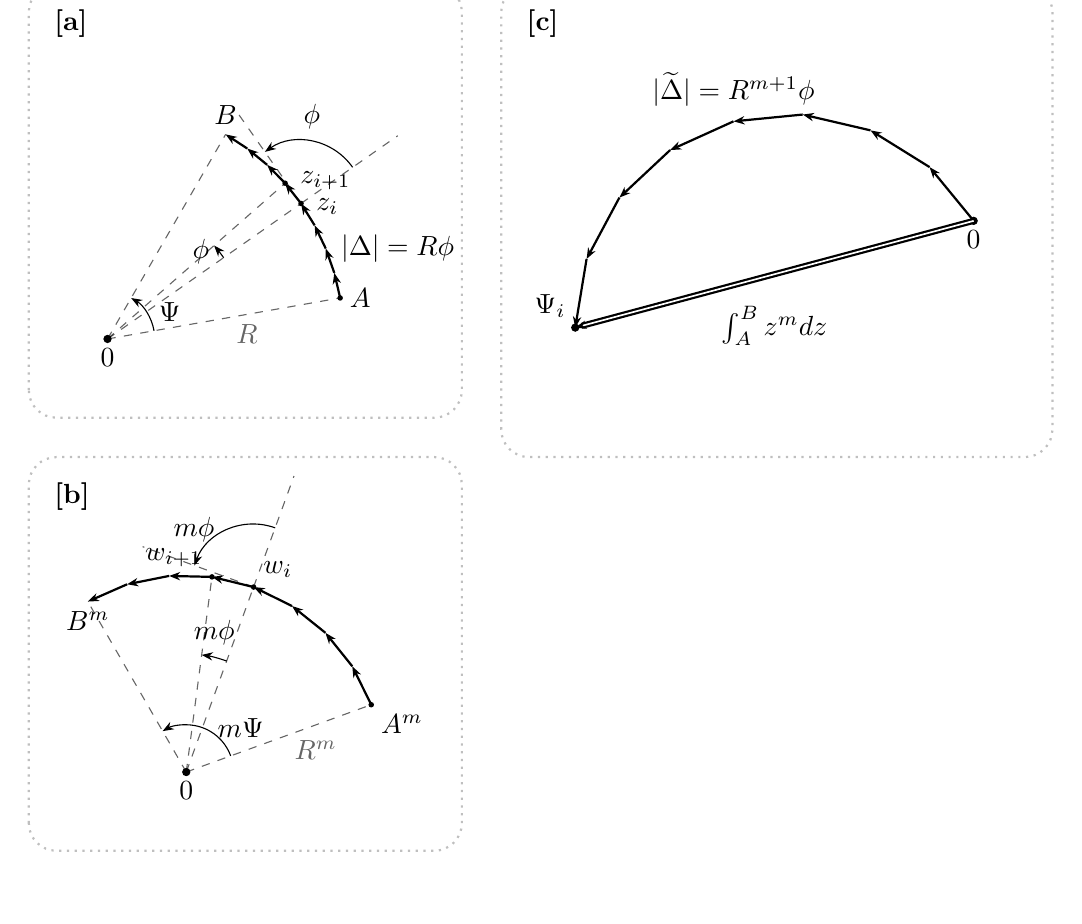
\begin{tikzpicture}[
        >={Stealth[length=4pt,width=3pt]},
        vector/.style={thick, ->},
        help line/.style={dashed, opacity=0.6},
        box/.style={draw=gray!50, rounded corners=10pt, dotted, thick}
      ]

      \def\R{3}
      \def\M{2}
      \def\StartAng{10}
      \def\EndAng{60}
      \def\Steps{8}

      \pgfmathsetmacro{\dAng}{(\EndAng-\StartAng)/\Steps}
      \pgfmathsetmacro{\dAngRad}{\dAng * pi / 180}
      \pgfmathsetmacro{\VecLen}{\R^(\M+1) * \dAngRad} % z^m \Delta z 的恒定长度

      % Panel [a]: 原始 z 平面上的路径和 \Delta z
      \draw[box] (-1,-1) rectangle (4.5, 4.5);
      \node[right, font=\bfseries] at (-0.8, 4) {[a]};

      \coordinate (O_a) at (0,0);
      \fill (O_a) circle (1.5pt) node[below] {$0$};

      \draw[help line] (O_a) -- (\StartAng:\R) node[pos=0.6, below] {$R$};
      \draw[help line] (O_a) -- (\EndAng:\R);
      \draw[->] (O_a) ++(\StartAng:0.6) arc (\StartAng:\EndAng:0.6)
      node[midway, right=1pt] {$\Psi$};

      \coordinate (PrevZ) at (\StartAng:\R);
      \fill (PrevZ) circle (1pt) node[right] {$A$};

      \foreach \k in {1,...,\Steps} {
        \pgfmathsetmacro{\tA}{\StartAng + (\k-1)*\dAng}
        \pgfmathsetmacro{\tB}{\StartAng + \k*\dAng}
        \coordinate (NextZ) at (\tB:\R);
        \draw[vector] (PrevZ) -- (NextZ);

        \ifnum\k=5
        \fill (PrevZ) circle (1pt) node[below=1pt, right=2pt] {$z_i$};
        \fill (NextZ) circle (1pt) node[above=1pt, right=2pt] {$z_{i+1}$};
        \draw[help line] (O_a) -- (PrevZ);
        \draw[help line] (O_a) -- (NextZ);
        \draw[->] (O_a) ++(\tA:1.8) arc (\tA:\tB:1.8) node[midway,
        left] {$\phi$};
        \draw[help line] (PrevZ) -- ($(PrevZ) + (\tA:1.5)$);
        \draw[help line] (PrevZ) -- ($(PrevZ) + (\tA+90:1.5)$);
        \draw[->] ($(PrevZ) + (\tA:0.8)$) arc (\tA:\tA+90:0.8)
        node[midway,above=1pt] {$\phi$};
        \fi

        \ifnum\k=3
        \node[right=2pt] at (PrevZ) {$|\Delta| = R\phi$};
        \fi

        \coordinate (PrevZ) at (NextZ);
      }
      \node[above] at (PrevZ) {$B$};

      % Panel [b]
      \begin{scope}[yshift=-5cm]
        \draw[box] (-1,-1.5) rectangle (4.5, 3.5);
        \node[right, font=\bfseries] at (-0.8, 3) {[b]};

        \coordinate (O_b) at (1,-0.5);
        \fill (O_b) circle (1.5pt) node[below] {$0$};

        \def\Rm{2.5}
        \pgfmathsetmacro{\WStartAng}{\M*\StartAng}
        \pgfmathsetmacro{\WEndAng}{\M*\EndAng}
        \pgfmathsetmacro{\WdAng}{(\WEndAng-\WStartAng)/\Steps}

        \draw[help line] (O_b) -- ($(O_b) + (\WStartAng:\Rm)$) node[pos=0.7,
        below=2pt] {$R^m$};
        \draw[help line] (O_b) -- ($(O_b) + (\WEndAng:\Rm)$);
        \draw[->] (O_b) ++(\WStartAng:0.6) arc
        (\WStartAng:\WEndAng:0.6) node[midway, right=2pt] {$m\Psi$};

        \coordinate (PrevW) at ($(O_b) + (\WStartAng:\Rm)$);
        \fill (PrevW) circle (1pt) node[below right] {$A^m$};

        \foreach \k in {1,...,\Steps} {
          \pgfmathsetmacro{\tA}{\WStartAng + (\k-1)*\WdAng}
          \pgfmathsetmacro{\tB}{\WStartAng + \k*\WdAng}
          \coordinate (NextW) at ($(O_b) + (\tB:\Rm)$);
          \draw[vector] (PrevW) -- (NextW);

          \ifnum\k=5
          \fill (PrevW) circle (1pt) node[above right] {$w_i$};
          \fill (NextW) circle (1pt) node[above left] {$w_{i+1}$};
          \draw[help line] (O_b) -- (PrevW);
          \draw[help line] (O_b) -- (NextW);
          \draw[->] (O_b) ++(\tA:1.5) arc (\tA:\tB:1.5) node[midway,
          above=1pt] {$m\phi$};
          \draw[help line] (PrevW) -- ($(PrevW) + (\tA:1.5)$);
          \draw[help line] (PrevW) -- ($(PrevW) + (\tA+90:1.5)$);
          \draw[->] ($(PrevW) + (\tA:0.8)$) arc (\tA:\tA+90:0.8)
          node[midway, left=1pt] {$m\phi$};
          \fi
          \coordinate (PrevW) at (NextW);
        }
        \node[below] at ($(O_b) + (\WEndAng:\Rm)$) {$B^m$};
      \end{scope}

      % Panel [c]
      \begin{scope}[xshift=7.5cm, yshift=-1.5cm]
        \draw[box] (-2.5,0) rectangle (4.5, 6);
        \node[right, font=\bfseries] at (-2.3, 5.5) {[c]};

        \coordinate (O_c) at (3.5,3);
        \fill (O_c) circle (1.5pt) node[below] {$0$};

        \coordinate (PrevS) at (O_c);

        \foreach \k in {1,...,\Steps} {
          \pgfmathsetmacro{\thetaK}{\StartAng + (\k-0.5)*\dAng}
          \pgfmathsetmacro{\vecAng}{(\M+1)*\thetaK + 90}

          \coordinate (NextS) at ($(PrevS) + (\vecAng:\VecLen*0.3)$);
          \draw[vector] (PrevS) -- (NextS);

          \ifnum\k=5
          \node[above=2pt] at (PrevS) {$|\widetilde{\Delta}| = R^{m+1}\phi$};
          \fi

          \coordinate (PrevS) at (NextS);
        }
        \fill (PrevS) circle (1.5pt) node[above left] {$\Psi_i$};

        \draw[vector, double, thick] (O_c) -- (PrevS) node[midway,
        below=8pt] {$\int_A^B z^m dz$};

      \end{scope}

    \end{tikzpicture}
  \end{center}

  \vspace{1em}
  Consider the Riemann sum $\sum_{i=1}^{n} z_i^m \Delta z_i$ where
  $z_i = Re^{i\theta_i}$ lies on the arc of radius $R$. Then the
  differential step is:
  \[
    \Delta z_i \approx iRe^{i\theta_i}\Delta\theta
  \]
  Multiplying $z_i^m$ and $\Delta z_i$, we have:
  \[
    z_i^m \Delta z_i \approx iR^{m+1}e^{i(m+1)\theta_i}\Delta\theta
  \]
  This can be viewed as an arc displacement along a circle of radius
  $\frac{R^{m+1}}{m+1}$ at angle $(m+1)\theta_i$, incrementing by
  $(m+1)\Delta\theta$. By accumulating these tangential vectors
  head-to-tail as depicted in Panel [c], the sum approximates an arc
  connecting $\frac{A^{m+1}}{m+1}$ and $\frac{B^{m+1}}{m+1}$ relative
  to the origin. The total resultant vector corresponds to the chord
  between these two points. Hence:
  \[
    \int_A^B z^m dz = \frac{1}{m+1}(B^{m+1} - A^{m+1})
  \]

\end{solution}

\section{Exercise 3.21}

Give a geometric interpretation of $\int_A^B e^z dz$ where the
integral is on the vertical segment $\gamma(t) = A + it$ with $t \in
[0, \theta]$, where $B = A + i\theta$ and $\theta > 0$. Then deduce the formula
\[
  \int_A^B e^z dz = e^B - e^A.
\]

\begin{proof}
  The plot is as below:
  \begin{center}

    \begin{tikzpicture}[
        >={Stealth[length=4pt,width=3pt]},
        vector/.style={thick, ->},
        help line/.style={dashed, opacity=0.6},
        box/.style={draw=gray!50, rounded corners=10pt, dotted, thick}
      ]

      \def\XA{1.5}
      \def\YA{0.5}       % r
      \def\Theta{2}      % \theta
      \def\Steps{10}
      \pgfmathsetmacro\dY{\Theta/\Steps}
      \pgfmathsetmacro\dAng{\dY * 180 / pi}
      \pgfmathsetmacro\StartAng{\YA * 180 / pi}
      \pgfmathsetmacro\EndAng{(\YA+\Theta) * 180 / pi}
      \def\Rw{2.5} % mapping radius for visual e^a

      % Panel [a]
      \begin{scope}[yshift=0cm]
        \draw[box] (-2,-1) rectangle (4.5, 4.5);
        \node[right, font=\bfseries] at (-1.8, 4) {[a]};

        \coordinate (O_a) at (0,0);
        \fill (O_a) circle (1.5pt) node[below left] {$0$};

        \draw[help line, ->] (-1.5,0) -- (2.5,0) node[right] {Re};
        \draw[help line, ->] (0,-0.5) -- (0,4) node[above] {Im};

        \coordinate (A_a) at (\XA, \YA);
        \coordinate (B_a) at (\XA, \YA + \Theta);
        \fill (A_a) circle (1.5pt) node[right] {$A$};

        \draw[help line] (A_a) -- (\XA, 0) node[below] {$a$};
        \draw[help line] (A_a) -- (0, \YA) node[left] {$b$};
        \draw[help line] (B_a) -- (0, \YA + \Theta) node[left] {$b+\theta$};

        \coordinate (PrevZ) at (A_a);

        \foreach \k in {1,...,\Steps} {
          \coordinate (NextZ) at (\XA, \YA + \k*\dY);
          \draw[vector] (PrevZ) -- (NextZ);

          \ifnum\k=3
          \node[right=2pt] at (PrevZ) {$|\Delta z| = \phi$};
          \fill (PrevZ) circle (1pt) node[left] {$z_i$};
          \fill (NextZ) circle (1pt) node[left] {$z_{i+1}$};
          \fi

          \coordinate (PrevZ) at (NextZ);
        }
        \fill (B_a) circle (1.5pt) node[right] {$B$};
      \end{scope}

      % Panel [b]
      \begin{scope}[yshift=-5.5cm]
        \draw[box] (-2,-1.5) rectangle (4.5, 4);
        \node[right, font=\bfseries] at (-1.8, 3.5) {[b]};

        \coordinate (O_b) at (1,0);
        \fill (O_b) circle (1.5pt) node[below left] {$0$};

        \draw[help line] (O_b) -- ($ (O_b) + (\StartAng:\Rw) $)
        node[pos=0.6, below
        right] {$e^a$};
        \draw[help line] (O_b) -- ($ (O_b) + (\EndAng:\Rw) $);

        \draw[help line] (O_b) -- ($ (O_b) + (0:\Rw)$);
        \draw[->] (O_b) ++(\StartAng:0.6) arc (\StartAng:\EndAng:0.6)
        node[midway, right=1pt] {$\theta$};
        \draw[->] (O_b) ++(0:0.4) arc (0:\StartAng:0.4) node[midway,
        right] {$b$};

        \coordinate (PrevW) at ($ (O_b) + (\StartAng:\Rw) $);
        \fill (PrevW) circle (1.5pt) node[right] {$e^A$};

        \foreach \k in {1,...,\Steps} {
          \pgfmathsetmacro\tA{\StartAng + (\k-1)*\dAng}
          \pgfmathsetmacro\tB{\StartAng + \k*\dAng}
          \coordinate (NextW) at ($ (O_b) + (\tB:\Rw) $);
          \draw[vector] (PrevW) -- (NextW);

          \ifnum\k=3
          \fill (PrevW) circle (1pt) node[below right] {$w_i$};
          \fill (NextW) circle (1pt) node[left] {$w_{i+1}$};
          \draw[help line] (O_b) -- (PrevW);
          \draw[help line] (O_b) -- (NextW);
          \draw[->] (O_b) ++(\tA:1.5) arc (\tA:\tB:1.5) node[midway,
          right] {$\phi$};
          \fi
          \coordinate (PrevW) at (NextW);
        }
        \fill (PrevW) circle (1.5pt) node[above] {$e^B$};
      \end{scope}

      % Panel [c]
      \begin{scope}[xshift=8cm, yshift=0.5cm]
        \draw[box] (-3,-3) rectangle (4.5, 4);
        \node[right, font=\bfseries] at (-2.8, 3.5) {[c]};

        \coordinate (O_c) at (3,0);
        \fill (O_c) circle (1.5pt) node[below right] {$0$};

        \coordinate (CenterC) at ($ (O_c) - (\StartAng:\Rw) $);

        \coordinate (PrevS) at (O_c);

        \foreach \k in {1,...,\Steps} {
          \pgfmathsetmacro\curAng{\StartAng + (\k-0.5)*\dAng}
          \pgfmathsetmacro\vecAng{\curAng + 90}
          \pgfmathsetmacro\stepLen{\Rw * \dY}

          \coordinate (NextS) at ($(PrevS) + (\vecAng:\stepLen)$);
          \draw[vector] (PrevS) -- (NextS);

          \ifnum\k=3
          \node[above right=2pt] at (PrevS) {$|\widetilde{\Delta}| = e^a \phi$};
          \fi
          \coordinate (PrevS) at (NextS);
        }
        \fill (PrevS) circle (1.5pt) node[above left] {$e^B - e^A$};

        \draw[vector, double, thick] (O_c) -- (PrevS) node[midway,
        below right] {$\int_A^B e^z dz$};

        \draw[help line, ->] (CenterC) ++(\StartAng:\Rw) arc
        (\StartAng:\EndAng:\Rw);
        \draw[help line] (CenterC) -- (O_c);
        \draw[help line] (CenterC) -- (PrevS);
        \fill (CenterC) circle (1pt) node[left] {$-e^A$};
      \end{scope}
    \end{tikzpicture}
  \end{center}

  \vspace{1em}

  Consider the Riemann sum $\sum_{i=1}^{n} e^{z_i}\Delta z_i$ where
  $A = a+ib$ and $B = a+i(b+\theta)$. The segment of length
  $\theta$ on $\text{Re}(z) = a$ maps to an arc of radius $e^a$
  from angle $b$ to $b+\theta$. Each step satisfies $\Delta z_i =
  i\phi$, so we have:
  \[
    e^{z_i}\Delta z_i = e^{z_i}(i\phi)
  \]
  which corresponds to an orthogonal step of size $e^a\phi$ along
  the tangential direction of the arc, as depicted in Panel [c].
  Connecting these vectors head-to-tail, the total displacement
  leads from $0$ to $e^B - e^A$. Hence:
  \[
    \int_A^B e^z dz = e^B - e^A
  \]

\end{proof}

\section{Exercise 3.22}

In Corollary 3.17, we computed the integral $\oint_\gamma \zeta^n
d\zeta$ for all integers $n$, where $\gamma$ is a circle centered at
the origin with positive orientation. Without invoking the Cauchy
integral theorem, calculate $\oint_\gamma \zeta^n d\zeta$ where
\begin{enumerate}
  \item[(a)] $\gamma$ is any circle not enclosing the origin;
  \item[(b)] $\gamma$ is a positively oriented square with vertices
    at $\pm 1 \pm i$.
\end{enumerate}

\begin{proof}
  Let $I_n(\gamma):=\oint_\gamma \zeta^n\,\dd\zeta$ for $n\in\mathbb{Z}$.

  For $n\neq -1$ we can use the primitive
  \[
    F_n(\zeta)=\frac{\zeta^{n+1}}{n+1},\qquad F_n'(\zeta)=\zeta^n,
  \]
  on every point of the curve (for $n\ge 0$, $F_n$ is entire; for
    $n\le -2$, $F_n$ is holomorphic on $\C\setminus\{0\}$, and the
  given curves do not pass through $0$). Hence for every closed
  piecewise smooth curve $\gamma$,
  \[
    I_n(\gamma)=0,\qquad n\neq -1.
  \]
  So only $n=-1$ remains.

  \begin{enumerate}
    \item[(a)] Let $\gamma$ be a positively oriented circle not enclosing
      $0$, say
      \[
        \gamma(t)=c+Re^{it},\quad t\in[0,2\pi],\quad |c|>R.
      \]
      Then
      \[
        I_{-1}(\gamma)
        =\int_0^{2\pi}\frac{iRe^{it}}{c+Re^{it}}\,\dd t
        =iR\int_0^{2\pi}\frac{e^{it}}{c}\cdot\frac{1}{1+(R/c)e^{it}}\,\dd t.
      \]
      Since $|R/c|<1$,
      \[
        \frac{1}{1+(R/c)e^{it}}=\sum_{k=0}^{\infty}(-1)^k\Bigl(\frac{R}{c}\Bigr)^k
        e^{ikt}
      \]
      uniformly in $t$, so
      \[
        I_{-1}(\gamma)
        =\frac{iR}{c}\sum_{k=0}^{\infty}(-1)^k\Bigl(\frac{R}{c}\Bigr)^k
        \int_0^{2\pi}e^{i(k+1)t}\,\dd t=0.
      \]
      Therefore,
      \[
        \oint_\gamma \zeta^n\,\dd\zeta=0\quad\text{for all }n\in\mathbb{Z}.
      \]

    \item[(b)] Let $\gamma$ be the positively oriented square with vertices
      $\pm1\pm i$. As above, for $n\neq -1$, $I_n(\gamma)=0$. For
      $n=-1$, split into four edges:

      \[
        \begin{aligned}
          &\gamma_1:\ z=1+it,\ t\in[-1,1],
          &&I_1=\int_{-1}^{1}\frac{i}{1+it}\,\dd t
          =\int_{-1}^{1}\frac{t-i}{1+t^2}\,\dd t=\frac{\pi i}{2},\\
          &\gamma_2:\ z=t+i,\ t\in[1,-1],
          &&I_2=\int_{1}^{-1}\frac{1}{t+i}\,\dd t
          =\int_{1}^{-1}\frac{t-i}{1+t^2}\,\dd t=\frac{\pi i}{2},\\
          &\gamma_3:\ z=-1+it,\ t\in[1,-1],
          &&I_3=\int_{1}^{-1}\frac{i}{-1+it}\,\dd t
          =\int_{1}^{-1}\frac{t-i}{1+t^2}\,\dd t=\frac{\pi i}{2},\\
          &\gamma_4:\ z=t-i,\ t\in[-1,1],
          &&I_4=\int_{-1}^{1}\frac{1}{t-i}\,\dd t
          =\int_{-1}^{1}\frac{t+i}{1+t^2}\,\dd t=\frac{\pi i}{2}.
        \end{aligned}
      \]
      Hence
      \[
        I_{-1}(\gamma)=I_1+I_2+I_3+I_4=2\pi i.
      \]
      Therefore,
      \[
        \oint_\gamma \zeta^n\,\dd\zeta=
        \begin{cases}
          2\pi i, & n=-1,\\
          0, & n\neq -1.
        \end{cases}
      \]
      in particular for this square.
  \end{enumerate}
\end{proof}

\section{Exercise 3.23}

For the counterclockwise oriented circle $\gamma(t) = r\exp(it)$ with
$t \in [0, 2\pi]$ and $r \in (|a|, |b|)$, prove
\[
  \oint_\gamma \frac{1}{(\zeta - a)(\zeta - b)} d\zeta = \frac{2\pi i}{a - b}.
\]
Hint: express $\frac{1}{\zeta - a}$ as the geometric series expansion
$\frac{1}{1-z} = \sum_{n=0}^\infty z^n$ for $|z| < 1$.

\begin{proof}
  Since $r\in(|a|,|b|)$, we have $|a|<r<|b|$. On $|\zeta|=r$,
  decompose
  \[
    \frac{1}{(\zeta-a)(\zeta-b)}
    =\frac{1}{a-b}\left(\frac{1}{\zeta-a}-\frac{1}{\zeta-b}\right).
  \]
  Hence
  \[
    \oint_\gamma \frac{1}{(\zeta-a)(\zeta-b)}\,\dd\zeta
    =\frac{1}{a-b}\left(
      \oint_\gamma\frac{1}{\zeta-a}\,\dd\zeta
      -
      \oint_\gamma\frac{1}{\zeta-b}\,\dd\zeta
    \right).
  \]

  For the first term, because $|a/\zeta|<1$ on $\gamma$,
  \[
    \frac{1}{\zeta-a}
    =\frac{1}{\zeta}\frac{1}{1-a/\zeta}
    =\sum_{n=0}^{\infty}a^n\zeta^{-n-1},
  \]
  uniformly on $\gamma$. Therefore we may integrate term-by-term:
  \[
    \oint_\gamma\frac{1}{\zeta-a}\,\dd\zeta
    =\sum_{n=0}^{\infty}a^n\oint_\gamma\zeta^{-n-1}\,\dd\zeta.
  \]
  By Exercise 3.22 (circle enclosing $0$), only $n=0$ contributes, so
  \[
    \oint_\gamma\frac{1}{\zeta-a}\,\dd\zeta=2\pi i.
  \]

  For the second term, because $|\zeta/b|<1$ on $\gamma$,
  \[
    \frac{1}{\zeta-b}
    =-\frac{1}{b}\frac{1}{1-\zeta/b}
    =-\sum_{n=0}^{\infty}\frac{\zeta^n}{b^{n+1}},
  \]
  uniformly on $\gamma$, hence
  \[
    \oint_\gamma\frac{1}{\zeta-b}\,\dd\zeta
    =-\sum_{n=0}^{\infty}\frac{1}{b^{n+1}}\oint_\gamma\zeta^n\,\dd\zeta=0,
  \]
  since $\oint_\gamma\zeta^n\,\dd\zeta=0$ for $n\ge0$.

  Combining both parts,
  \[
    \oint_\gamma \frac{1}{(\zeta-a)(\zeta-b)}\,\dd\zeta
    =\frac{1}{a-b}(2\pi i-0)
    =\frac{2\pi i}{a-b}.
  \]
\end{proof}

\end{document}
